\documentclass[journal]{IEEEtran}

\usepackage{cite}
\usepackage{graphicx}
\usepackage{amsmath}
\usepackage{algorithmic}

\begin{document}
\title{Political Districting via Discrete Particle Swarm Optimization}
\author{~David~Fu,~David~Zhang,~Ellen~Wang,~Leslie~Reyes,~Seikun~Kambashi,~Shiranka~Miskin}
\maketitle

\begin{abstract}
% The Summary should be a brief version of the full report. It should give the
% reader an accurate overview. Be brief, but be specific. 
The abstract goes here.
\end{abstract}

\section{Introduction}
% Summarize the importance of the problem you are trying to solve and the reason
% that motivated you to select this project. Explain what was the problem or
% challenge that you were given? state the purpose of the project and how did
% you solve it? Enumerate the objectives of the project and describe in brief
% the structure of the report. 
\IEEEPARstart{T}{his} demo file is intended to serve as a ``starter file''
for IEEE journal papers produced under \LaTeX\ using
IEEEtran.cls version 1.8b and later.
I wish you the best of success.


\section{Literature Review}
% Conduct a critical survey on similar solutions and explain how your solution
% extends or differs from these solutions. 

\section{Problem Formulation and Modeling}
% Include the problem statement and describe its model.
The Political Districting problem can be modeled as an assignment problem with specific constraints.  The goal is to assign a fixed set of Geographical Units (GUs) to a fixed number of districts, where each district is contiguous, while minimizing a certain cost function.  

Let $U$ be the set of all GUs, and let $D$ be the set of all districts.  Our goal is to minimize 
\begin{equation}
\sum_{u \in U} \sum_{d \in D} c_{ud} x_{ud}\\
\end{equation}
where
\begin{equation}
x_{ij} = 1 \text{ or } 0\\
\end{equation}
\begin{equation}
\sum_{d \in D} x_{ud} = 1, (u \in U)\\
\end{equation}


\section{Proposed Solution}
\subsection{Initial Solution}
% Generate an initial solution.
\subsection{Cost Function}
% Suggest a cost function (objective function) suitable for this problem.
While there are many factors that can be considered for political districting, for the sake of efficiency and simplicity, our fitness function only focuses on the two main goals of political districting which are population equality and district compactness.  These measures do not assess the contiguity of a solution, as the algorithms used are designed to only evaluate valid solutions.  A constant coefficient is introduced to each term to allow us to tune how much each factor contributes to the overall fitness.

$$f(x) = c_{pop} \cdot f_{pop} + c_{shape} \cdot f_{shape}$$

\subsubsection{Population Equality}
In an ideal solution, each district would have the same population, which would equal the average population across the districts.  We therefore define the measure of population equality for a set of districts $D$ where $P_d(x)$ is the total population of district $d \in D$ as
$$f_{pop}(x) = \sum_{d \in D} \left(P_d(x) - \frac{\sum_{j \in D} P_j(x)}{|D|}\right)$$

\subsubsection{Compactness}
To evaluate compactness we use the Schwartzberg Index, which is the perimeter of a district squared divided by its area, due to it being simple to compute.

$$f_{shape} = \sum_{d \in D} \frac{(perimeter_d)^2}{area_d}$$

\subsection{Neighborhood}
% Define a suitable neighborhood operator.
The neighborhood of a given solution is defined as all possible solutions reachable by swapping one GU from district $i$ to district $j$.  
\subsection{Algorithm Description}
% Define a suitable solving strategy for this problem.
\subsection{Parameter Values}
% Select your own values for the parameter and explain the basis for your selection.
\subsection{Example Runthrough}
% Describe how each algorithm (TS, SA, GA, PSO and ACO) will proceed to solve
% this problem by performing at least two hand iterations on a reduced version
% of the problem.
We will demonstrate two iterations of the three algorithms we have chosen to implement using a simple example input.
The input will be represented as a grid of cells, where each cell shares a border with its vertical and horizontal neighboring cells. 

The population of each cell will be assumed to be 1 for simplicity, and the solution will be a grouping of cells such that there are exactly two groups that represent two districts. \\

\subsubsection{Simulated Annealing}~\\\\
% \begin{figure}[h!]
%     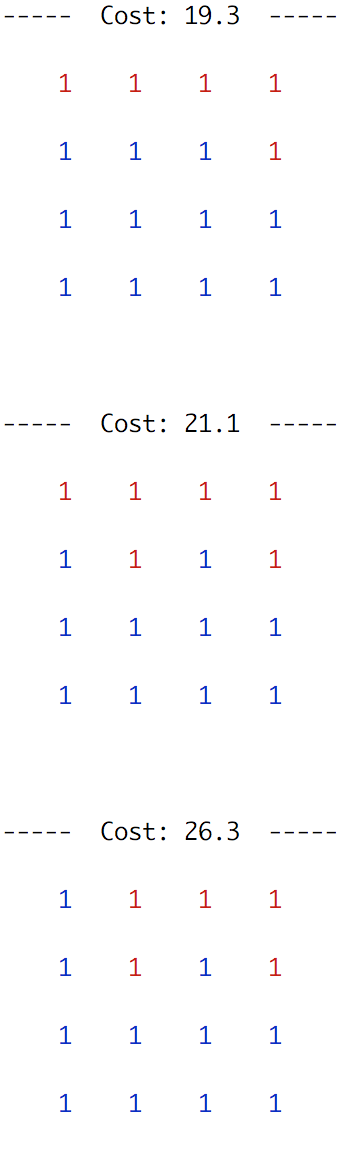
\includegraphics[width=3cm]{sa.png}
%     \centering
%     \label{fig:sa_example}
%     \caption{Example run using Simulated Annealing}
% \end{figure}
Figure \ref{fig:sa_example} shows the first two iterations of the SA implementation.
We start with a randomly generated initial solution of two districts with a fitness cost of 19.3 (calculated using the previously defined cost function).

The neighborhood of the initial solution is defined by the set of possible cell swaps (switching a cell from one district to another) without breaking continuity.

The algorithm will randomly pick one of these neighbors, and will choose it as the new solution if its fitness is better than the current one, or if the acceptance probability given the current temperature allows for worser solutions.

The algorithm does not stop in the first two iterations since the stopping conditions have not been met. Since the temperature is quite high in the beginning, the first two iterations also end up accepting solutions that have a worse fitness than the previous solution. \\

\subsubsection{Tabu Search}~\\\\
% \begin{figure}[h!]
%     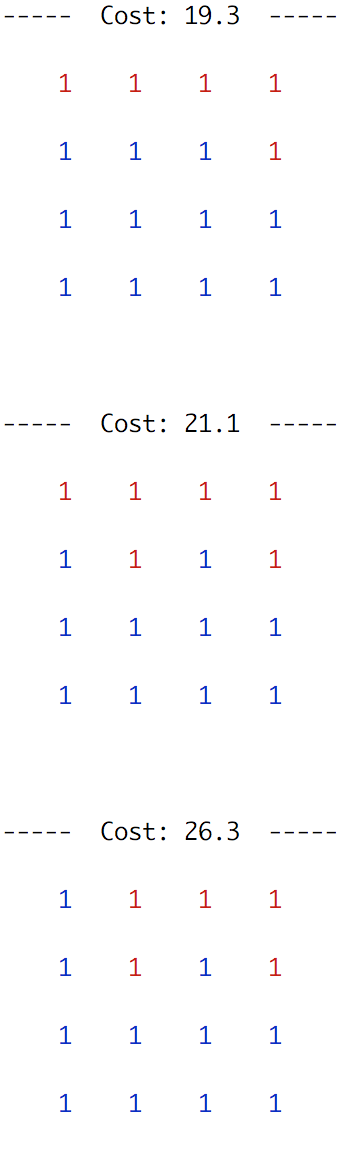
\includegraphics[width=3cm]{sa.png}
%     \centering
%     \label{fig:sa_example}
%     \caption{Example run using Tabu Search}
% \end{figure}


\section{Performance Evaluation}
Hello
% Establish a set of evaluation metrics and run some experiments with different
% values of algorithm parameters to quantitatively and qualitatively assess the
% performance of the developed solution using different meta-heuristic
% optimization techniques. Students must identify the pros and cons of each
% technique and assess the quality of work as well as its fit with project
% objectives.

\begin{table}[!h]
\centering
\caption{Compactness Results for 100 Iterations}
\label{comp_100iter}
\begin{tabular}{l|llll}
                       & \multicolumn{4}{l}{\textbf{Compactness}}                      \\ \hline
\textbf{Algorithm}     & \textbf{min} & \textbf{max} & \textbf{median} & \textbf{stdev} \\ \hline
\textbf{SA}            & 19.255       & 587.016      & 495.146         & 244.594       \\
\textbf{PSO}           & 57.213       & 229.580      & 109.956         & 33.041         \\
\textbf{Hill Climbing} & 52.983       & 264.8        & 122.061         & 41.088         \\
\textbf{Tabu Search}   & 66.946       & 257.239      & 127.855         & 39.242            
\end{tabular}
\end{table}

\begin{table}[!h]
\centering
\caption{Population Equality Results for 100 Iterations}
\label{pop_100iter}
\begin{tabular}{l|llll}
                       & \multicolumn{4}{l}{\textbf{Population Equality}}             \\ \hline
\textbf{Algorithm}     & \textbf{min} & \textbf{max} & \textbf{median} & \textbf{stdev} \\ \hline
\textbf{SA}            & 1841655      & 4648349.5    & 3098654         & 787073.096         \\
\textbf{PSO}           & 2463         & 94699        & 32829.25        & 15648.72           \\
\textbf{Hill Climbing} & 1749         & 218283       & 9859.75         & 28231.930        \\
\textbf{Tabu Search}   & 36195.5      & 9319.25         & 5647.456       & 5315.779     
\end{tabular}
\end{table}

\begin{table}[!h]
\centering
\caption{Overall Fitness Results for 100 Iterations}
\label{fitness_100iter}
\begin{tabular}{l|llll}
                       & \multicolumn{4}{l}{\textbf{Fitness}}                          \\ \hline
\textbf{Algorithm}     & \textbf{min} & \textbf{max} & \textbf{median} & \textbf{stdev} \\ \hline
\textbf{SA}            & 3683810.325  & 9296718.255  & 6197845.196     & 1573915.146    \\
\textbf{PSO}           & 5082.820     & 189513.077   & 65748.985       & 31296.346      \\
\textbf{Hill Climbing} & 3644.275     & 436675.159   & 19839.867       & 56463.519      \\
\textbf{Tabu Search}   & 5315.779     & 72478.096    & 18799.833       & 11289.642     
\end{tabular}
\end{table}

\section{Conclusions \& Recommendations}
% Summarize the conclusion and future improvement. Explain how did you solve the
% problem, what problems were met? what did the results show? And how to refine
% the proposed solution? You may organize ideas using lists or numbered points,
% if appropriate, but avoid making your report into a check-list or a series of
% encrypted notes 



\begin{thebibliography}{1}
% Every report needs references; in fact, your failure to consult
% references for guidance may be considered negligence. On the other
% hand, when you include sentences, photos, drawings or figures from
% other sources in your report, the complete reference must be cited.
% Failure to do so is plagiarism, an academic infraction with serious
% consequences.

\bibitem{tsp-pso}
Kang-Ping~Wang et al. Particle Swarm Optimization for Travelling Salesman
        Problem, 2003

\bibitem{voronoi}
Federica~Ricca et al. Weighted Voronoi region algorithms for political
        districting, 2008

\bibitem{local-search}
    Burcin~Bozkaya et al.  A tabu search heuristic and adaptive memory procedure
        for political districting, 2003
\end{thebibliography}
\end{document}



